% !TEX TS-program = xelatex
% !TEX encoding = UTF-8
\documentclass[12pt,oneside]{article}
% % % UTILITIES % % %
\usepackage{graphicx, color, url} %  \includegraphics  %  \colorbox{defined-color}{text}  %  \textcolor{defined-color}{text} or {\color{defined-color} text}
%\definecolor{lightGray}{gray}{0.8} \definecolor{midGray}{gray}{0.5} \definecolor{darkGray}{gray}{0.3} 
%EQUIVALENT: \definecolor{midGray}{rgb}{0.5,0.5,0.5} \definecolor{midGray}{RGB}{127,127,127} \definecolor{midGray}{HTML}{7F7F7F} 
\definecolor{urlGreen}{rgb}{0.1,0.5,0.1} \newcommand{\gurl}[1]{\urlstyle{same}\color{urlGreen}\url{#1}} % \newcommand{\furl}[1]{\urlstyle{same}\url{#1}}
\usepackage{natbib} % \citet{} = author (date), \citep[see]{} = (see author, date), \citealp & \citealt = no parens, \citep* & \citet* don't "et al", \citeyearpar
% % % FONTS % % %
\usepackage{fontspec} % call basic font defs with \textnormal{} \textsf{sans} \textrf{roman} \texttt{mono} \textbf{bold} \textsc{smallcap} \textit{italic}
%\setmainfont[Numbers={Lining}]{Linux Libertine O} %\setromanfont[Ligatures=TeX]{Charis SIL}  %\setsansfont{M+ 1c}  %\setmonofont{M+ 1m}
\setmainfont{FreeSerif} \setmonofont{FreeMono}
% \newfontfamily\code[]{FreeMonoBold} %EXAMPLE: The {\osf 24}th Annual...
%\defaultfontfeatures{Mapping=tex-text} % handles " (straight quotes) poorly
%\usepackage{xeCJK} \setCJKmainfont{UnBatang}  %\setCJKmainfont{AR PL UKai}  %\setCJKmainfont{AR PL UMing}  %\setCJKmainfont{WenQuanYi Zen Hei}  %\setCJKmainfont{UnDotum} %sans-Hanggul   %\XeTeXlinebreaklocale "zh"  \XeTeXlinebreakskip = 0pt plus 1pt
%\XeTeXinterchartokenstate=1 % enable codepoint-by-codepoint font mapping
%\XeTeXcharclass `\• 0 \XeTeXcharclass `\₀ 0 \XeTeXcharclass `\“ 0 \XeTeXcharclass `\” 0 \XeTeXcharclass `\‘ 0 \XeTeXcharclass `\’ 0
% alternate: \xeCJKsetcharclass{`\start}{`\end}{characterclass}, e.g., \xeCJKsetcharclass{`\₀}{`\₉}{1}
% % % LAYOUT % % %
\usepackage[letterpaper, margin=1in]{geometry} % smaller margins
\usepackage[auth-sc, affil-it]{authblk} % author/affiliation management
\usepackage[parfill]{parskip} % begin paragraphs with empty line, not an indent
\usepackage{enumitem, paralist} % ENUMITEM (list margin arguments): \begin{itemize}[leftmargin=2cm]  %PARALIST (inline enums/items): \asparaenum & \inparaenum
\newenvironment{itm}{\begin{itemize}[leftmargin=*]}{\end{itemize}}  % just like itemize, but with bullets flush left with surrounding text
\renewcommand{\labelitemi}{•} \renewcommand{\labelitemii}{◦} \renewcommand{\labelitemiii}{—} % redefine default bullets
\usepackage[compact]{titlesec} % control spacing before/after section titles
\titlespacing{\section}{0pt}{*2}{*-0.5} \titlespacing{\subsection}{0pt}{*0}{*0} \titlespacing{\subsubsection}{0pt}{*0}{*0} %{cmd}{Lmargin}{aboveskip}{belowskip}
%\usepackage{ragged2e, multicol} %RAGGED2E: \RaggedRight   %MULTICOLS: \begin{multicols}{2} ... \end{multicols}
\usepackage{minted, array, float, multicol} % listings
\usemintedstyle{default}
\usepackage{fancyhdr}
%\setlength{\topmargin}{-0.4in} \setlength{\headheight}{0.4in} \setlength{\headsep}{0.2in} \setlength{\textheight}{8.4in} \setlength{\footskip}{0.4in}
\pagestyle{fancy} \fancyhf{} 
%\renewcommand{\headrule}{\color{lightGray}\hrule width\headwidth height 0.75pt \vskip-\headrulewidth}
%\renewcommand{\footrule}{\color{lightGray}\hrule width\headwidth height 0pt \vskip-\footrulewidth}
\lhead[] {\fancyplain{}{\small{Technical Reports of the UW Linguistic Phonetics Laboratory}}}
\chead[] {\fancyplain{}{}}
\rhead[] {\fancyplain{}{\#2012-01}}
\lfoot[] {\fancyplain{}{}}
\cfoot[] {\fancyplain{}{\thepage}}
\rfoot[] {\fancyplain{}{}}
%\lstset{ language=R, basicstyle=\ttfamily, stepnumber=1, showspaces=false, showstringspaces=false, showtabs=false, frame=none, tabsize=2, captionpos=b, breaklines=true, breakatwhitespace=false, title=\lstname, escapeinside={}, keywordstyle={}, morekeywords={}, escapechar={}, breakindent=1em, breakautoindent} %ɪɛæɑɔʊʌ
%\usepackage{tablefootnote}
%\usepackage{fancyhdr} \pagestyle{fancy} \fancyhf{}
%\lhead[]{} \chead[]{} \rhead[]{} \lfoot[]{} \cfoot[]{\fancyplain{}{\osf \thepage}} \rfoot[]{}  %\cmd[oddpage]{evenpage}
% % % VARIOUS USEFUL UNICODE POINTS FOR COPY/PASTE % % %
% “” ‘’ — – ‣•◦ ◆◇■◼◾▪□◻◽▫▶▸▷▹๛ ¹²³⁴⁵⁶⁷⁸⁹⁰⁺⁻⁼⁽⁾ⁱⁿ₀₁₂₃₄₅₆₇₈₉₊₋₌₍₎ₐₑₒₓₔ ←↑→↓↔↕↚↛⇋⇌⇐⇑⇒⇓⇔⇕⇍⇏⇎⇠⇡⇢⇣⇦⇧⇨⇩⟵⟶⟷⟸⟹⟺   ∀ ∃ ∄ ∅ ∈ ∉ ⟦ ⟧ ⊂ ⊃ ⊆ ⊇ ⟨ ⟩ ⟪ ⟫ ≝ ∿ ≃ ≄ ≈ ≉ ≤ ≥ ≪ ≫ ≺ ≻ ⊀ ⊁ ≼ ≽ 𝒫
\title{Vowel normalization and plotting with the phonR~package\footnote{Development of the phonR package was funded in part by the National Institutes of Health, grant \# R01DC006014 to Pamela Souza. The author would like to thank August McGrath for her assistance in developing and debugging early versions of the \texttt{plotVowels} function.}\vspace{-1ex}}
\author{Daniel~R.~McCloy\\Department of Linguistics, University of Washington\\drmccloy@uw.edu\vspace{-1ex}}
\date{} % empty=no date, comment out to use current date
\begin{document}
\thispagestyle{plain}
\maketitle

\section{Introduction}
%\begin{multicols}{2}
The phonR package is a collection of functions for the R language \citep{r} intended to meet the needs of phoneticians and phonologists.  Currently the package includes functions for vowel normalization and vowel plotting; other functions for tasks like generating standard consonant charts and manipulating distinctive feature vectors for phone inventories are under development.  This document describes phonR's vowel plotting and normalization capabilities.

The vowel plotting capabilities in phonR were developed to enhance the flexibility and visual appeal of vowel plots, especially plots with multiple groups' data on a single graph.  To that end, several options are available in phonR that are unavailable or difficult to achieve with other vowel plotting tools (the vowels package in R \citep{vowelsR} and its associated website NORM \citep{norm} being a popular alternative).  In particular, the phonR package implements confidence interval plotting based on bivariate normal density contours, allowing for ellipsoids in F2×F1 space whose major and minor axes are not restricted to the horizontal or vertical (compare to NORM's crosshairs-style plotting of standard deviations in the F1 and F2 dimensions).  Additionally, phonR introduces support for automatic drawing of the vowel polygon as well as the option to leave certain vowels unconnected to the polygonal line (e.g., central vowels like [ə]).  Finally, both vowel means and individual vowel tokens may be plotted with IPA glyphs or geometric symbols (or may be omitted), with smart defaults for various color, linestyle, and shape options.

The phonR package can be downloaded from the Comprehensive R Archive Network ({\gurl http://cran.r-project.org/package=phonR}). The source code is hosted at {\gurl https://github.com/drammock/phonR}, and is released under GPL-3 ({\gurl http://www.gnu.org/licenses/gpl.html}).  The package's plotting functionality depends on two other R packages: mixtools \citep{mixtools} and Cairo \citep{cairoR}.  The Cairo R package in turn depends on the Cairo graphics library \citep{cairo}; installation of the Cairo graphics library is described in Section~\ref{sec:apx}.  Plotting with IPA glyphs instead of geometric shapes may also require a typeface with Unicode-IPA symbols; the package defaults to the Charis-SIL font \citep{charis}, but future versions will be more flexible regarding font choice.

Like all R packages, phonR can be installed from within R with the \texttt{install.packages} command.  Alternatively, downloaded source code can be installed from a command line console with the command \texttt{R CMD INSTALL phonR -l /path/to/unzipped/source/of/phonR/}, and some R frontends also have GUIs for package installation.  Regardless of installation method, the package is loaded with the R command \texttt{library(phonR)}.
%\end{multicols}

\section{Normalizing vowels with phonR}
%\begin{multicols}{2}
The phonR function \texttt{normalizeVowels} implements several of the most common normalization algorithms, which are listed in Table~\ref{tab:norms}.  Depending on the normalization method chosen, the function can operate on a single vector of values, or may require both F1 and F2 (Watt-Fabricius method) or all of f0, F1, F2, and F3 (Nearey-2 method).  Additionally, the Watt-Fabricius, Nearey-1, Nearey-2 and Lobanov normalization methods can make use of an optional argument \texttt{grouping.factor}, which allows normalization to occur speaker-intrinsically (other normalization methods are automatically speaker-intrinsic by virtue of their formulae).
%\end{multicols}

\begin{table}[htb]
	\begin{center}
		\begin{tabular}{>{\raggedright}p{10em} {l} >{\arraybackslash}{l}}
			\hline \\ [-0.5em]
			\textbf{Normalization method}            & \textbf{Source}           & \textbf{Formula}\\ [0.25em] \hline \\ [-0.25em]
			Bark                                      & \citet{traunmuller1990}   & \(\displaystyle \frac {26.81 \times F_n}{1960+F_n} - 0.53 \) \\  [1.5em]
			Equivalent Rectangular Bandwidth (erb)    & \citet{glasbergMoore1990} & \(\displaystyle 21.4 \times \log_{10} (1 + F_n \times 0.00437) \) \\ [1em]
			Mel                                       & \citet{mel}               & \(\displaystyle 2595 \times \log_{10} (1 + \frac{F_n}{700}) \) \\ [1em]
			Log                                       & n/a                        & \(\displaystyle \log_{10}(F_n) \) \\ [1.5em]
			Lobanov (z‑transform, z‑score)             & \citet{lobanov1971}       & \(\displaystyle \frac{F_n - \mu(F_n)}{\sigma(F_n)} \) \\ [2em]
			Watt-Fabricius (s‑centroid)\footnotemark & \citet{wattFabricius2002} & \(\displaystyle \frac{F_n}{centroid} \) \\ [2em]
			Nearey‑1 (logmean)                         & \citet{nearey1977}        & \(\displaystyle \log_{e} (F_n) - \mu(\log_{e}(F_n)) \) \\ [1em]
			Nearey‑2                                   & \citet{nearey1977}        & \(\displaystyle \log_{e}(F_n) - \sum_{n=0}^{3} \mu(\log_{e}(F_n)) \) \\ [1em] \hline
		\end{tabular}
	\end{center}
	\caption{Normalization methods available via phonR's \texttt{normalizeVowels} function}
	\label{tab:norms}
\end{table}
\footnotetext{In the phonR package, the centroid is defined as the point \( \langle \frac{\min(\overline{F2_{vowel}})+\max(\overline{F2_{vowel}})}{2}, \frac{2 \times \min(\overline{F1_{vowel}})+\max(\overline{F1_{vowel}})}{3} \rangle \).  This varies slightly from the formula in \citet{wattFabricius2002}, since the phonR implementation simply calculates which vowel has the highest mean F1 value and designates it as low corner of the triangle, rather than asking the user to expressly specify the \textit{trap} or \textit{start} vowel. Similarly, the phonR implementation simply calculates which vowel has the highest mean F2 value and uses that to calculate the upper left corner, rather than expressly looking for the mean of the “point-vowel” /i/.  The upper right corner is, as in the original method, derived from the other two.}

\section{Generating vowel plots with phonR}
%\begin{multicols}{2}
The comprehensive function call for vowel plotting is shown in Listing~\ref{lst:comp}, and the resulting plot is shown in Figure~\ref{fig:indoMaximal}.  Of special note here are the arguments \texttt{match.axes}, \texttt{poly.order}, and \texttt{poly.include}.  The first of these, \texttt{match.axes}, determines whether all graphs will have the same axis limits; possible values are \texttt{'absolute'} (all graphs have the same dimensions), \texttt{'relative'} (all graphs have the same scale and aspect ratio, but their absolute limits may vary), or \texttt{'none'} (graphs may vary in their scale, aspect ratio, and/or absolute limits).  This argument applies only when a grouping factor is supplied and \texttt{single.plot=FALSE}, so it was ignored when drawing the plot in Figure~\ref{fig:indoMaximal}, but the effect of \texttt{match.axes='absolute'} (the default value) can be seen in Figure~\ref{fig:indoLattice}.  
%\end{multicols}

\begin{listing}[bth]
\begin{minted}[samepage, fontsize=\small, formatcom=\bfseries]{r}
plotVowels(data=myDataFrame, f1='F1_column_name', f2='F2_column_name', 
  f3='F3_column_name', f0='f0_column_name', vowel='Vowel_column_name', 
  grouping.factor='Gender_column_name', norm.method='mel', match.unit=
  TRUE, match.axes='absolute', points='shape', points.alpha=0.3, 
  means='text', means.alpha=1, ignore.hidden=TRUE, ellipses=TRUE, 
  ellipse.size=0.3173, polygon=TRUE, poly.order=c('i','e','a','o','u'), 
  poly.include=NULL, single.plot=TRUE, axis.col='#666666FF', titles=
  'auto', grayscale=FALSE, vary.shapes=TRUE, vary.lines=TRUE, legend=
  TRUE, uniform.style=FALSE, aspect.ratio=NULL, plot.dims=c(6.5,6.5), 
  plot.unit='in', output='pdf')
\end{minted}
\caption{A comprehensive function call to phonR's \texttt{plotVowels} function}
\label{lst:comp}
\end{listing}

%\begin{multicols}{2}
The \texttt{poly.order} argument specifies the order in which vowels should be connected if \texttt{polygon=TRUE}; the default value for this argument is the set \{i, ɪ, e, ɛ, æ, a, ɑ, ɔ, o, ʊ, u, ʌ\}, and it is only necessary to explicitly provide this argument if you prefer the polygon be drawn in a different order or if your data contains vowels not in the default set.  The \texttt{poly.include} argument takes an integer indicating how many of the vowels present in the data should be connected by the polygon segments, allowing certain vowels to be omitted (for example, one might choose to connect only the short vowel in a series of long/short vowel pairs, in which case the long vowels should be placed at the end of the \texttt{poly.order} vector, and \texttt{poly.include} should be the index of the last vowel to be connected to the polygonal line).  Also shown in Figure~\ref{fig:indoMaximal} is the automatic axis labeling with regard to the chosen normalization method, variation in plot symbol shape and linestyle, and the effect of the transparency arguments (\texttt{points.alpha} and \texttt{means.alpha}).  The line styles cycle through the default linestyles in R, but the plot symbols are restricted to a subset of the symbols available through \texttt{pch}, namely the set ○ □ △ ◇ ● ■ ▲ ◆ + × ▽. % ✛ ⨯

A more typical function call includes fewer arguments, as in Listing~\ref{lst:typ}; the output of this function call is shown in Figure~\ref{fig:indoOverlay}.  This example illustrates a few of the intelligent defaults of phonR's \texttt{plotVowels} function.  For example, graphical options like line style or shape are automatically held constant if the plot is in color, or if each subject/group is plotted on a separate graph.  Listing~\ref{lst:typ} also illustrates that the \texttt{data} argument may be omitted if the other required inputs are supplied as separate vectors (note the lack of quotation marks on the \texttt{f1}, \texttt{f2}, \texttt{vowel}, and \texttt{grouping.factor} arguments).  
%\end{multicols}

\begin{figure}[H]
	\begin{center}
		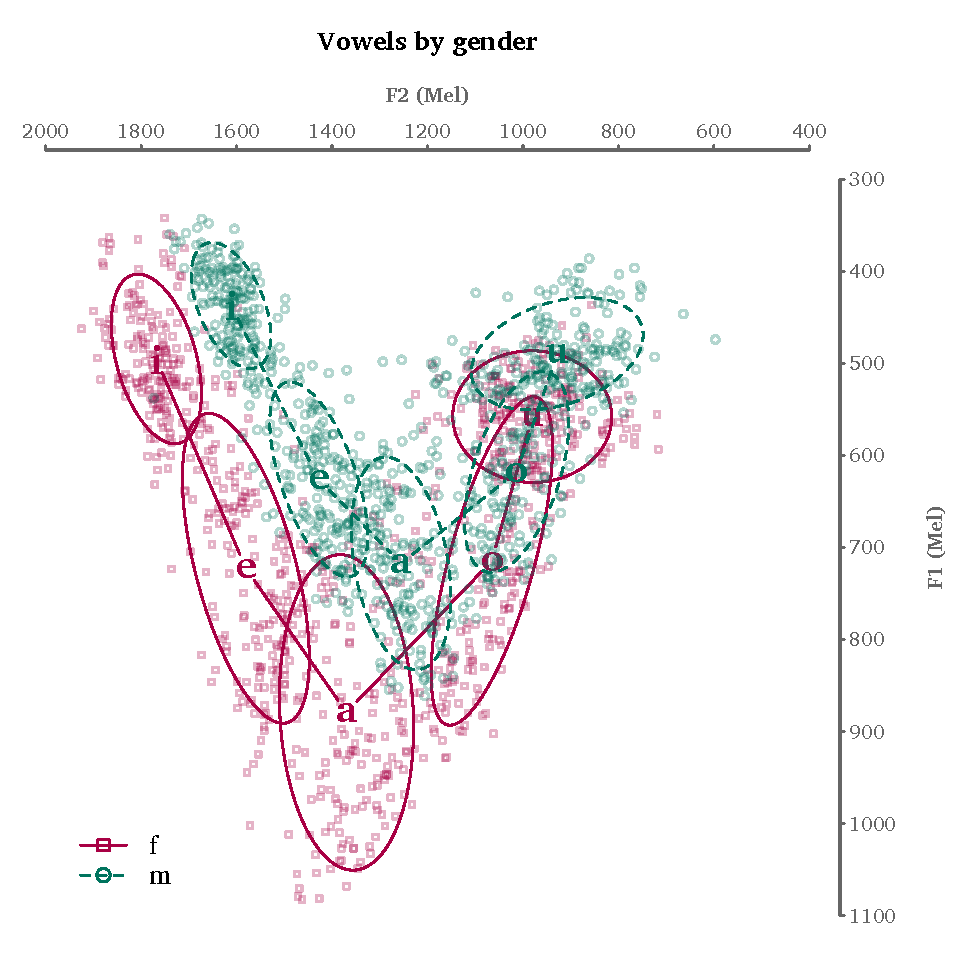
\includegraphics[keepaspectratio=true,scale=1]{indoMaximal.pdf} %[width=\textwidth]
		\caption{Vowel plot based on the maximal function call in Listing~\ref{lst:comp}}
		\label{fig:indoMaximal}
	\end{center}
\end{figure}

%\begin{multicols}{2}
For colored plots, \texttt{plotVowels} generates colors of equal chroma and luminance, with hues equally spaced around the color circle in HCL space \citep{hcl}.  A custom title is also included here; the \texttt{titles} argument accepts either a string or vector of strings, and will recycle or discard strings as needed (with a warning to the user) if there is a mismatch between the number of graphs to be generated and the number of strings provided.  Finally, Figure~\ref{fig:indoOverlay} illustrates the \texttt{match.unit=FALSE} argument, which transforms the data points using the specified normalization method (in this case, the Bark transformation) and plots them in the transformed space, but labels the axes with values equispaced in Hz, highlighting the non-linearity of the transform (note the unequal spacing of tickmarks that are numerically equidistant).
%\end{multicols}

\begin{listing}[tbh]
\begin{minted}[samepage, fontsize=\small, formatcom=\bfseries]{r}
plotVowels(data=myDataFrame, f1='F1_column_name', f2='F2_column_name', 
  vowel='Vowel_column_name', grouping.factor='subj', norm.method=
  'bark', match.unit=FALSE, points='none', points.alpha=0.6, means=
  'text', means.alpha=1, ignore.hidden=TRUE, ellipses=FALSE, polygon=
  TRUE, single.plot=TRUE, grayscale=FALSE, legend=TRUE, titles=
  'Indonesian vowel spaces (means and polygons)', aspect.ratio=1.5, 
  plot.dims=c(6.5,6.5), plot.unit='in', output='pdf')
\end{minted}
\caption{A typical function call to phonR's \texttt{plotVowels} function}
\label{lst:typ}
\end{listing}

\begin{figure}[H]
	\begin{center}
		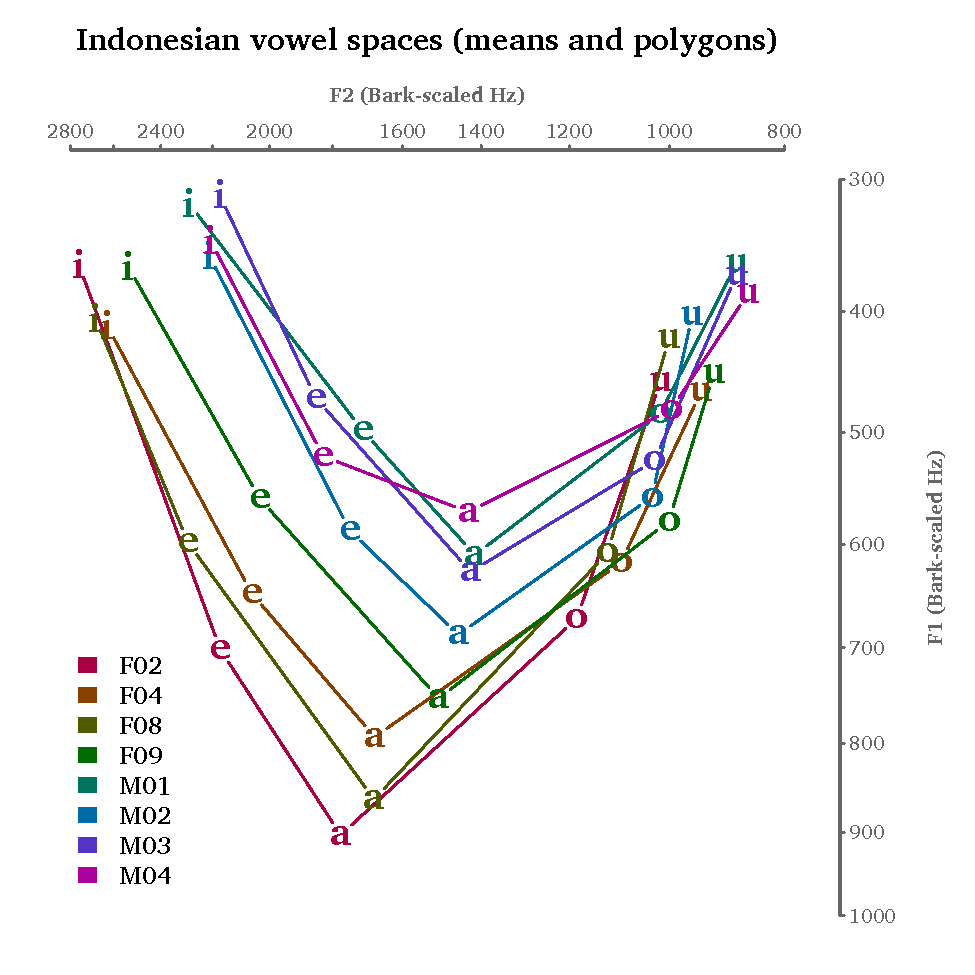
\includegraphics[width=\textwidth]{indoOverlay.pdf}
		\caption{Vowel plot based on the typical function call in Listing~\ref{lst:typ}}
		\label{fig:indoOverlay}
	\end{center}
\end{figure}

%\begin{multicols}{2}
A minimal function call may include only \texttt{f1}, \texttt{f2}, and \texttt{vowel} arguments. The four main plot elements (points, means, ellipses, and polygons) each have default values and thus may be omitted if the defaults are suitable; omitting \texttt{grouping.factor} treats all points as belonging to the same subject or group.
%\end{multicols}

\begin{listing}[H]
\begin{minted}[samepage, fontsize=\small, formatcom=\bfseries]{r}
plotVowels(f1=f1Vector, f2=f2Vector, vowel=vowelVector, 
  grouping.factor=groupingVector, points='none', means='text', 
  ellipses=TRUE, polygon=TRUE, single.plot=FALSE, output='screen')
\end{minted}
\caption{A minimal function call to phonR's \texttt{plotVowels} function}
\label{lst:min}
\end{listing}

\begin{figure}[H]
	\begin{center}
		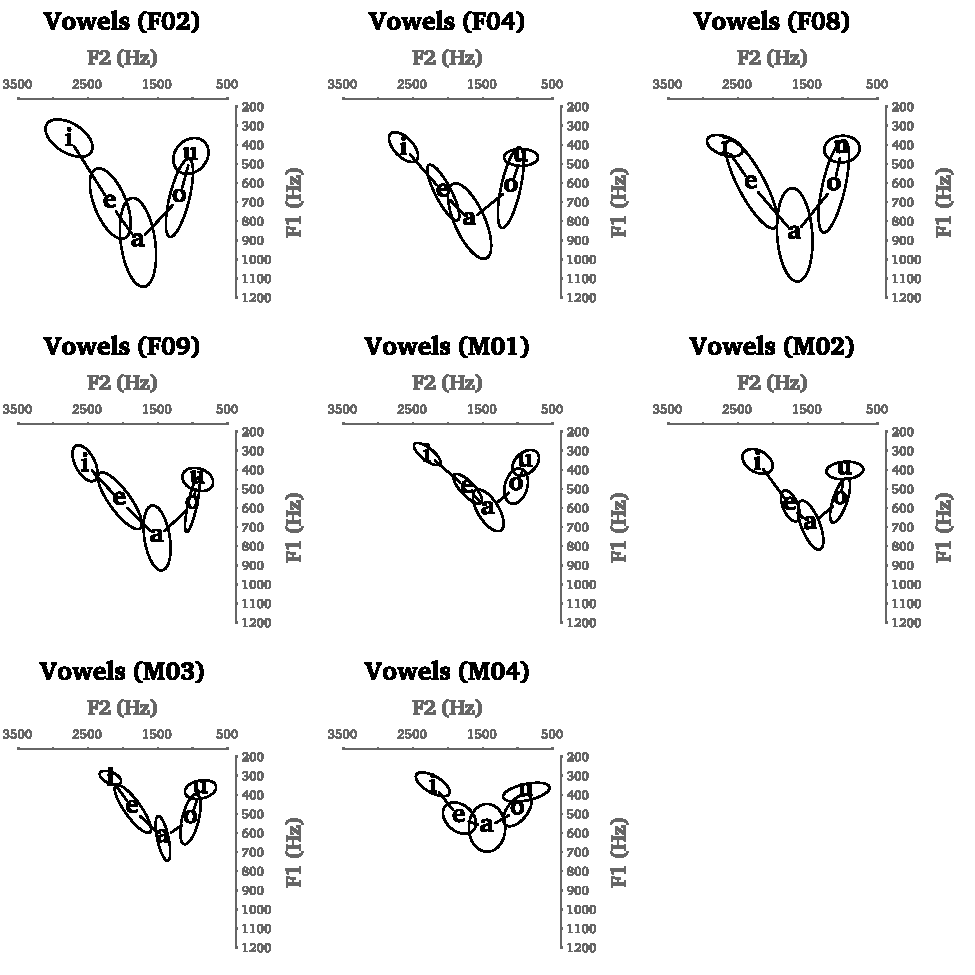
\includegraphics[width=\textwidth]{indoLattice.pdf}
		\caption{Vowel plot based on the minimal function call in Listing~\ref{lst:min}}
		\label{fig:indoLattice}
	\end{center}
\end{figure}

%\begin{multicols}{2}
Listing~\ref{lst:min} and its corresponding plot in Figure~\ref{fig:indoLattice} show another unique feature of the \texttt{plotVowels} function, which is that the argument \texttt{single.plot=FALSE} behaves differently depending on output method.  If the output method is \texttt{'pdf'} or \texttt{'jpg'}, then a separate PDF or JPG file will be created for each group.  In contrast, if the output method is \texttt{'screen'} then the graphs for each group are arranged in a grid so they can be easily inspected side-by-side.  It also illustrates the automatic titling functionality, which labels each graph with the grouping factor value (in this case, subject number, though this could just as easily be task type, dialect, ethnicity, etc).  Finally, as mentioned above, Figure~\ref{fig:indoLattice} illustrates the effect of the argument \texttt{match.axes='absolute'}, which forces all graphs to the same dimensions and axis limits, allowing visual comparisons between graphs of the relative size and position of different speakers' vowel spaces. 
%\end{multicols}

\section{Appendix: Installing the Cairo graphics library}
\label{sec:apx}
%\begin{multicols}{2}
Most versions of Linux distribute the Cairo graphics library through standard package management systems, and in most cases Cairo will already be installed.  On Ubuntu-like systems you should check for the presence of packages “libcairo2” and “libcairo2-dev”.  On OS-X, installing Cairo is trivially accomplished through either Fink or MacPorts (though I'm told the installation of MacPorts itself is sometimes finicky).  See {\gurl http://www.cairographics.org/download/} for instructions.  Getting the Cairo graphics library to work on Windows is tricky, and the guidance on the Cairo Graphics website was incomplete at time of writing.  A method that is known to work is to download the run-time files from the GTK website and manually move them to the proper folder within your R system install path.  Specifically, go to {\gurl http://www.gtk.org/download/} and click on “Windows” (either 32-bit or 64-bit depending on your computer).  Then scroll down to “Required third party dependencies” and download the run-time files for \texttt{zlib}, \texttt{cairo}, \texttt{libpng}, \texttt{fontconfig}, \texttt{freetype}, and \texttt{expat}.  Uncompress them and gather up all the DLL files from the “bin” folders that were in each zipped package.  Then move/copy those DLL files into the \texttt{/bin/x64/} folder\footnote{or on 32-bit systems, the \texttt{/bin/i386/} folder.} within your R program directory (usually this is C:/Program Files/R/R-2.14.0 or similar).  Also move or copy “fonts.conf” from the \texttt{fontconfig} zip file, and put that into the \texttt{/etc/x64/fonts/} folder\footnote{or on 32-bit systems, the \texttt{/etc/i386/fonts/} folder.} within the R program directory.  Of course, you will still need to install the Cairo R package from within R to make use of these libraries for plotting.
%\end{multicols}

% % % BIBLIOGRAPHY  % % %
\newpage
\bibliography{phonR}
\bibliographystyle{apa-good}   %\bibliographystyle{apalike}   %\bibliographystyle{plain}
\end{document}
